%%%%%%%%%%%%%%%%%%%%%%%%%%%%%%%%%%%%%%%%%%%%%%%%%%%%%%%%%%%%%%%%%%%%%%%%
\begin{frame}[t]{[LF59] 5-Band User EQ}
\begin{tiny}
\begin{tabular}{@{}lccc@{}}
\toprule
Function & Off/On & Option & Specification \\
\midrule
Audio EQ & \color{black}{Off} & Instart &
\multirow{10}{60mm}{
\begin{itemize}
\item Frequency Response Check
	\begin{itemize}
	\item 100Hz, 300Hz, 1kHz, 3kHz, 10kHz에서 +10과 -10에서의 출력레벨과 ref와의 출력레벨 차이값이 4dBr 이상
	\end{itemize}
\end{itemize}
} \\
Sound Engine & \color{blue}{On} & Instart & \\
Clearvoice & \color{black}{Off} & & \\
Autovolume & \color{black}{Off} & & \\
Surround & \color{black}{Off} & & \\
Smart Sound & \color{black}{Off} & & \\
3D Sound Zooming & \color{black}{Off} & & \\
Sound Mode & \color{blue}{On} & \color{blue}{User EQ±10} & \\
Sound Optimizer & \color{black}{Off} & & \\
OSD Volume & \color{blue}{On} & Vol.40 & \\
\midrule
\end{tabular}
\end{tiny}

\begin{figure}[b]
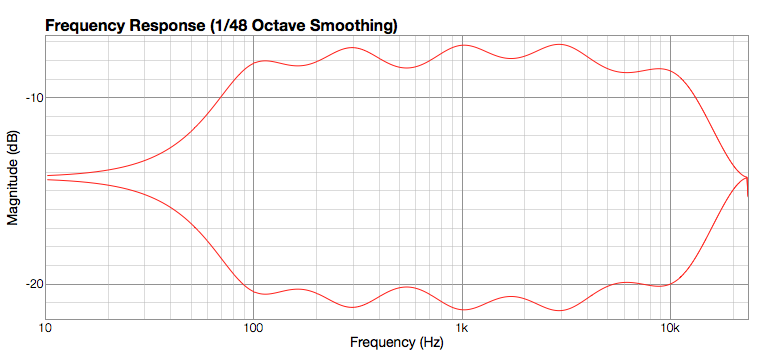
\includegraphics[height=0.4\textwidth]{figures/5_band_user_eq.png}
\end{figure}

\end{frame}
